\section{Introduction}
\label{sec:intro}

Recent advancements in video large language models (video-LLMs)~\cite{tang2025video, cheng2025vilamp} have demonstrated significant capabilities in video understanding and reasoning. In contrast to image large language models (image-LLMs)~\cite{Kwai2025Keye-VL, coreteam2025mimovltechnicalreport}, which focus on static visual content analysis, video-LLMs must capture dynamic visual information across frames. This demands robust temporal understanding, a critical research challenge that has garnered substantial attention in recent work~\cite{Cheng2025V-STaR,Song2025Video-MMLU}.

\begin{figure}[htbp]
    \centering
    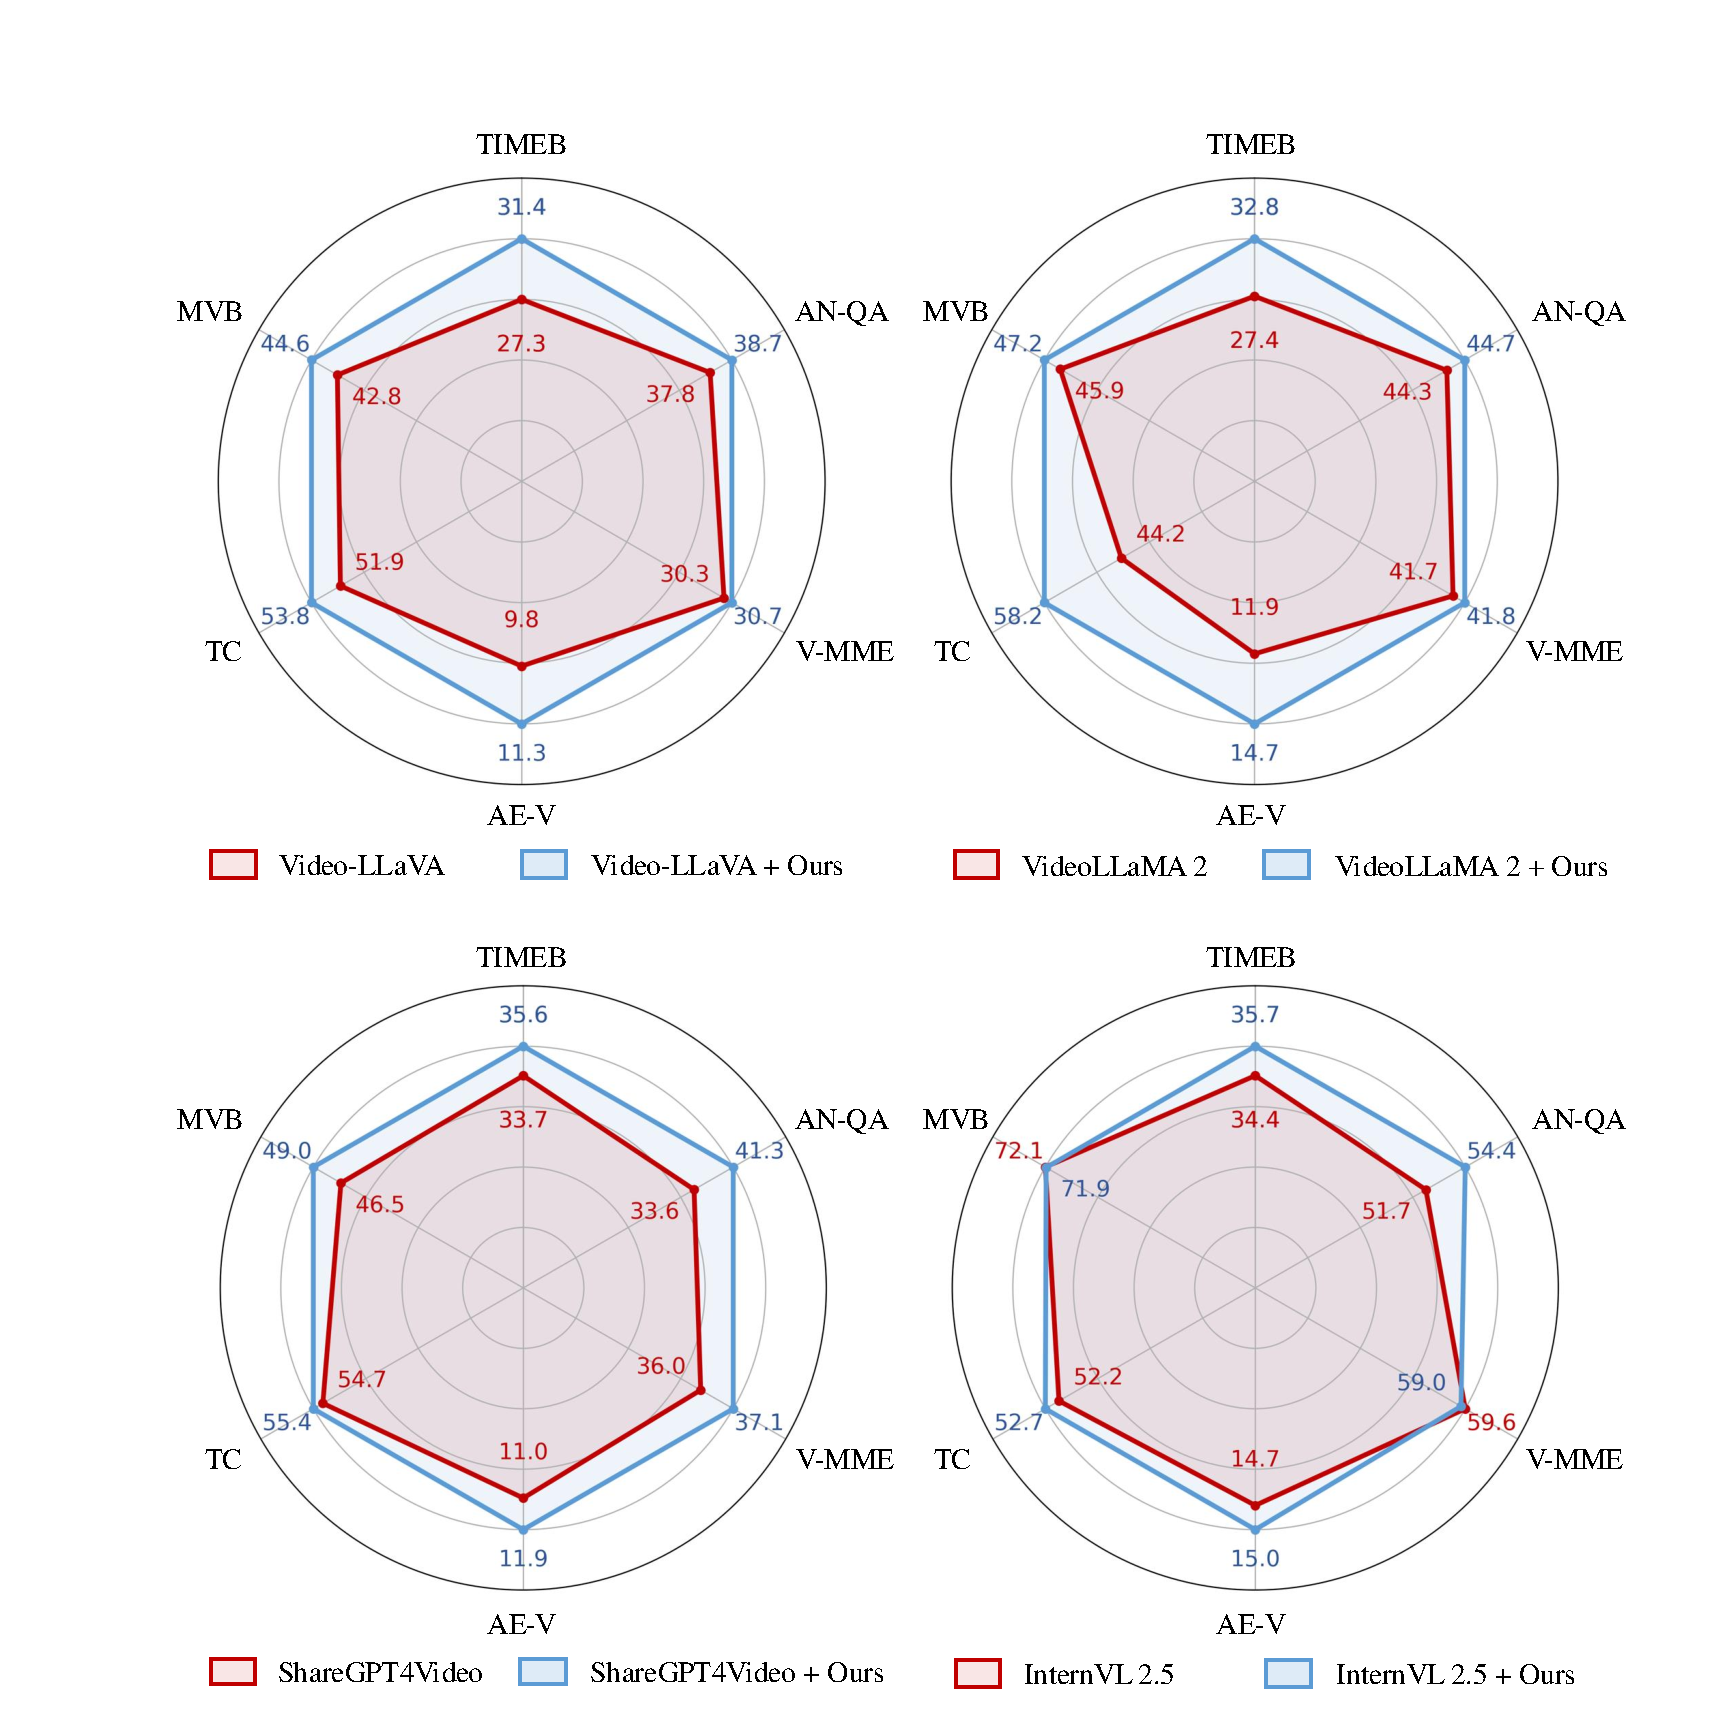
\includegraphics[width=1.0\linewidth]{radar.pdf}
    
    \caption{Performance of four video-LLMs evaluated across six benchmarks. ``+ Ours'' suffix denotes models fine-tuned with our approach, achieving substantial improvements on all benchmarks. TIMEBench (TIMEB), MVBench (MVB), TempCompass (TC), and AutoEval-Video (AE-V) focus on temporal scenarios, whereas Video-MME (V-MME) and ActivityNet-QA (AN-QA) evaluate general performance.}
    \label{fig:radar}
\end{figure}

Despite efforts to enhance temporal understanding in video-LLMs~\cite{Cheng2024VideoLLaMA, Liu2024ST-LLM}, recent studies indicate that significant challenges remain in tasks requiring advanced temporal reasoning~\cite{Wang2024VideoHallucer, Xiao2025VideoQA}. These limitations can be attributed to the following primary factors: \textbf{1) Insufficient temporal instruction fine-tuning data.} Current video instruction tuning datasets~\cite{Lin2024Video-LLaVA, Chen2024ShareGPT4Video} prioritize generalization across common scenarios rather than in-depth temporal comprehension. Although some approaches, such as AVicuna~\cite{Tang2024AVicuna}, generate temporal instruction tuning datasets through video splicing, their applicability remains limited to temporal localization due to the inherent constraints of this method. \textbf{2) Exploitation of data shortcuts.} For instance, in determining a child's movement direction (e.g., the \textit{Dynamic} dimension in Figure~\ref{fig:tasks}), models may rely on facial orientation instead of conducting a genuine temporal analysis of positional changes, leading to errors when videos are reversed. Notably, temporal benchmarks~\cite{Li2024MVBench,Liu2024TempCompass} are also affected by such shortcuts. Our experimental results (Figure~\ref{fig:benchmark}) show that performance based on single random frames significantly surpasses random baselines, indicating that many questions can be resolved without true temporal reasoning, thereby overestimating model capabilities.

\begin{figure*}[htbp]
    \centering
    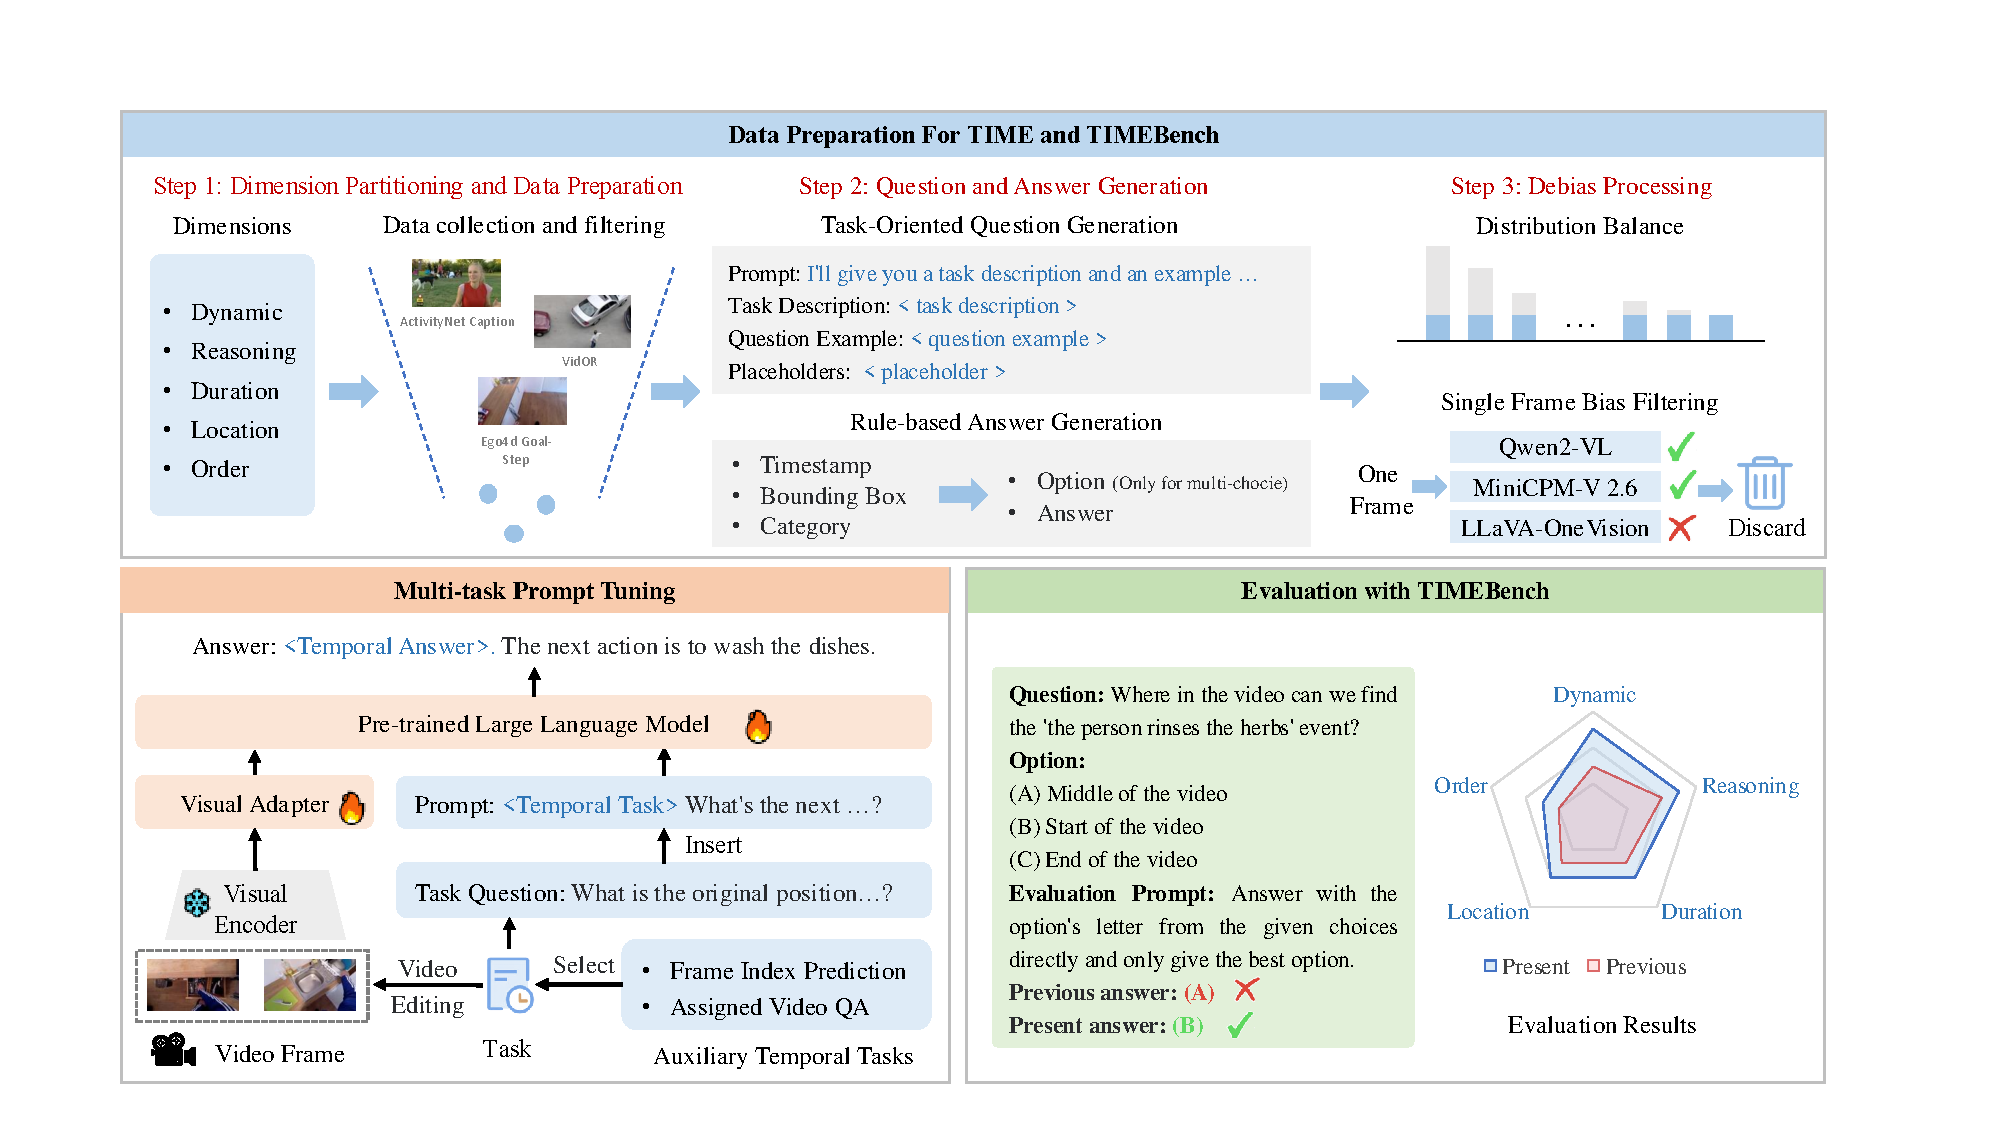
\includegraphics[width=0.85\linewidth]{pipeline.pdf}
    \caption{Overall framework overview. Our approach comprises three key components: the TIME instruction tuning dataset, the multi-task prompt tuning approach, and the TIMEBench video temporal understanding benchmark. The top panel shows the data preparation flow for TIME and TIMEBench in three sub-steps.  The bottom left illustrates the multi-task prompt tuning, where auxiliary temporal tasks are randomly interleaved with the original prompt, enabling the model to address additional temporal tasks alongside the main question.  The bottom right displays the evaluation format in TIMEBench, with all questions in a multiple-choice format for objective evaluation. }
    \label{fig:pipeline}
\end{figure*}

To address these challenges, we systematically enhance Video-LLMs' temporal understanding and evaluation through the following improvements. First, \textbf{we construct a Temporal-sensItive Multi-dimEnsional (TIME) instruction-tuning dataset} comprising 34,000 carefully curated samples across five key temporal dimensions (including \textit{Dynamic}, \textit{Reasoning}, \textit{Duration}, \textit{Location}, and \textit{Order}), which serves as a valuable complement to existing general-purpose instruction-tuning datasets. These dimensions capture essential aspects of temporal reasoning, such as the dynamics of events over time and the capacity to predict future occurrences. Simultaneously, we implement rigorous data filtering to remove any potential data shortcuts that might undermine the effectiveness of model tuning. Second, to further mitigate limitations in data volume, \textbf{we propose a Multi-Task Prompt tuning (MTP) framework} that augments standard instruction tuning with two types of temporal-oriented self-supervised tasks: frame-level task to improve single-frame temporal understanding, and segment-level task to enhance cross-segment temporal understanding. As shown in Figure~\ref{fig:radar}, fine-tuning with our approach results in substantial performance gains across most temporal benchmarks for the evaluated video-LLMs. Finally, \textbf{we develop a robust Temporal-sensItive Multi-dimEnsional Benchmark (TIMEBench)}, which covers five dimensions of temporal evaluation and provides a more accurate measure of temporal understanding ability by filtering out potential data shortcuts through a carefully designed filtering mechanism. Experimental results validate the rigor of our evaluation benchmark.

   
In summation, our contributions are as follows:
\begin{itemize}
    \item We construct a temporal-sensitive  multi-dimensional instruction-tuning dataset intended to augment existing general instruction-tuning corpora, incorporating curated samples that specifically address temporal reasoning challenges in video data.
    
    \item We introduce a novel multi-task prompt-tuning approach that enhances existing instruction fine-tuning processes with two temporal-oriented self-supervised tasks. 

    \item We propose a robust temporal-sensitive  multi-dimensional benchmark that provides a more accurate measure of temporal understanding ability by filtering out potential data shortcuts.

\end{itemize}



